\documentclass[a4paper,12pt]{article}

%% Definitioner för vågfysikrapporten-dokument

%% Text-kodning, språk samt PS-font
\usepackage[utf8]{inputenc}
\usepackage[T1]{fontenc}
\usepackage{ae,aecompl}
\usepackage{listings}
% % bitmap-grafik
\usepackage{graphicx}
% % matematik
\usepackage{amsmath}
\usepackage{mathtools}
\usepackage{latexsym}
\usepackage{graphicx}

%% Paragrafformat
\setlength{\parindent}{0pt}
\setlength{\parskip}{1ex plus 0.5ex minus 0.2ex}

%% Format för datum
\newcommand{\twodigit}[1]{\ifthenelse{#1<10}{0}{}{#1}}
\newcommand{\dagensdatum}{
\number\year-\twodigit{\number\month}-\twodigit{\number\day}}

%% Sidhuvud och sidfot
\usepackage{fancyhdr}
\pagestyle{fancy}
\lhead{Alexander Poole}
\chead{INLÄMNINGSUPPGIFT 1-1080}
\rhead{TSEA05}
\lfoot{alepo020@student.liu.se}
\cfoot{{\ } \\ \thepage}
\rfoot{19920829-0057}

%%Title
\title{TSEA05 \\ INLÄMNINGSUPPGIFT 1-1080}
\author{Alexander Poole}

%%Gray box
\usepackage{mdframed}


%%Dokumentets början
\begin{document}
\maketitle
\thispagestyle{empty}
\newpage

%%TODO
\section*{Problemformulering}
Målet med uppgiften är att ta det givna enborten A-B i figur \ref{fig:original} och förenkla det till dess Theveninekvivalenta eller Nortonekvivalenta motsvarighet, se figur \ref{}. För att åstakomma detta får Ohms lag, KCL, KVL samt slinganalys, nodanalys eller metoden med incidensmatriser användas.

\section*{Lösning}
Problemet löses med hjälp av slinganalys.

\begin{figure}[h]
\centering
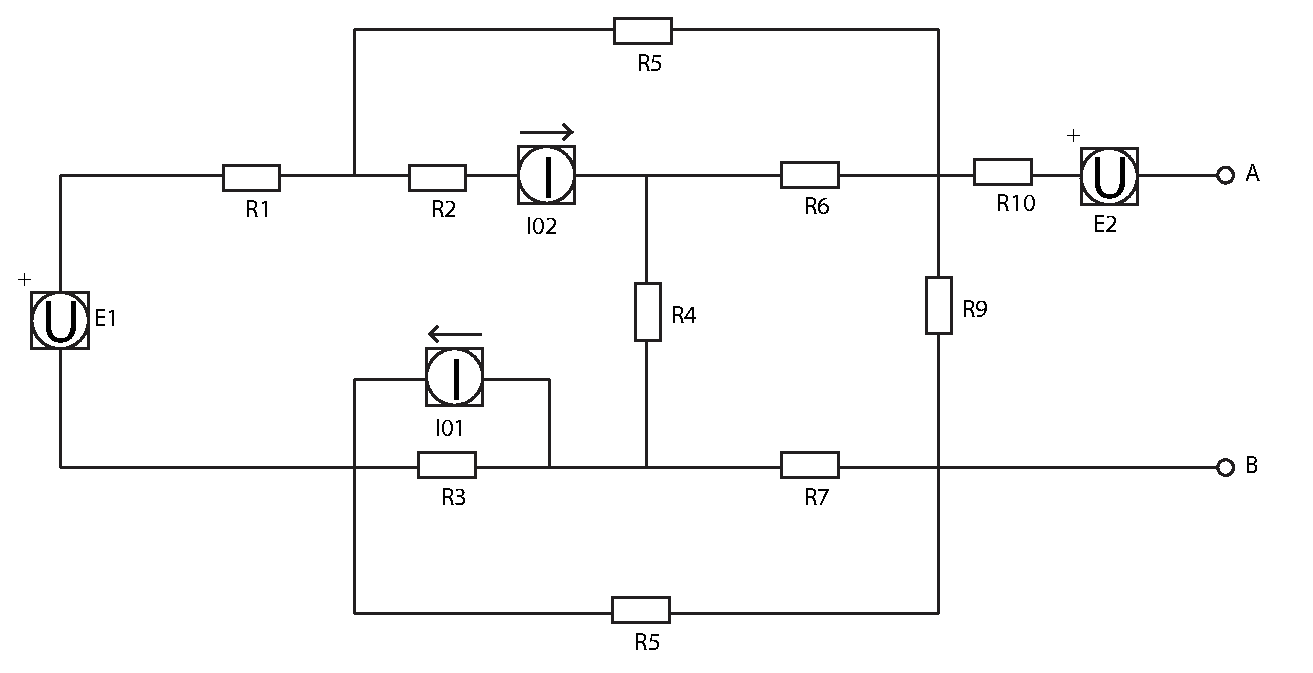
\includegraphics[width=1\textwidth]{bilder/originalnat.eps}
\caption{Nät givet i uppgiften.}
\label{fig:original}
\end{figure}

Föränklar bort R2 ty i serie med strömkällan I02. Förenklar bort den ensamma strömkällan I02. Sätter in strömmar i de slingor som uppstår, samt kortsluter enporten A-B för att kunna bestämma kortslutnings strömmen, se \ref{fig:modnat}.

\begin{figure}[h]
\centering
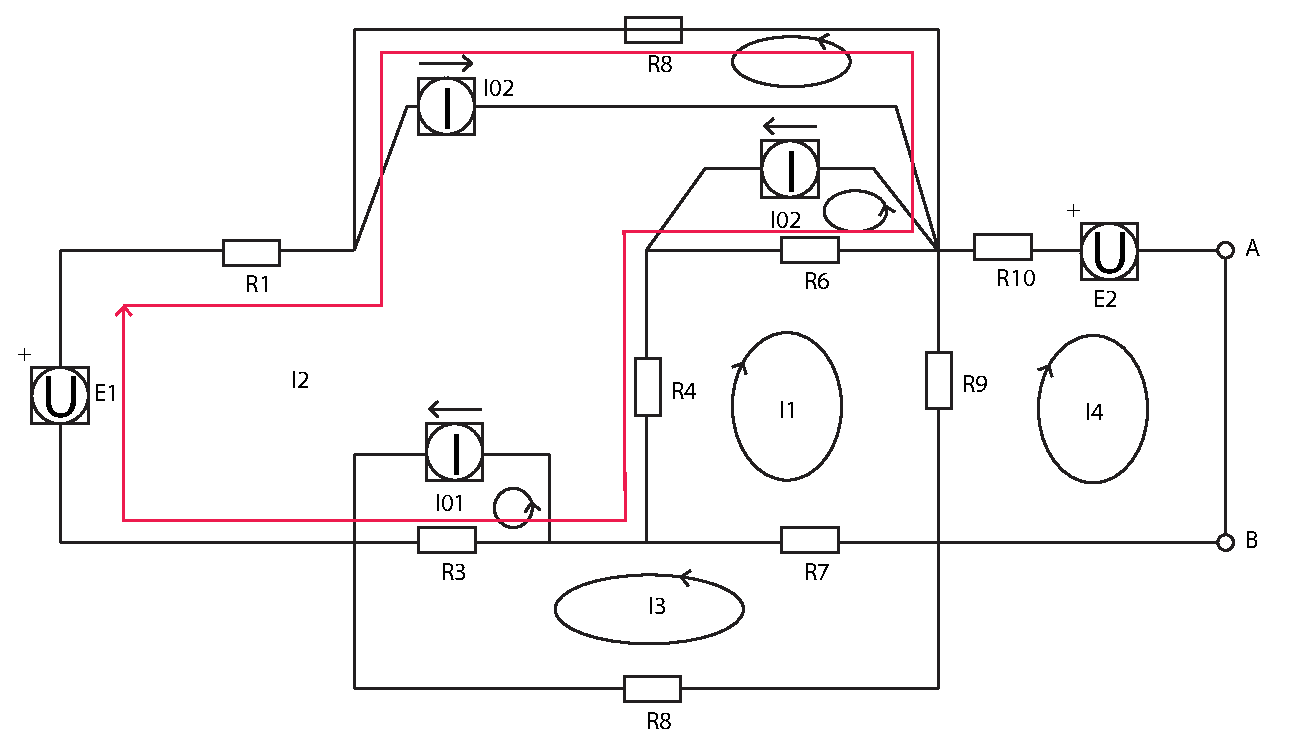
\includegraphics[width=1\textwidth]{bilder/modnat.eps}
\caption{Nät efter förenklingar, med angivna slingor och strömmar.}
\label{fig:modnat}
\end{figure}

KVL annvänds på samtliga slingor detta ger ekvation \ref{ekv:I1}.

\begin{equation}
\text{I1: }-R_7(I_1+I_3)-R_4(I_1-I_2)-R_6(I_1-I_2+I_{02})-R_9(I_1-I_4)=0 \\
\label{ekv:I1}
\end{equation}

\begin{equation}
\text{I2: }-R_1I_2-R_8(I_2-I_{02})-R_6(I_2-I_1-I_{02})-R_4(I_2-I_1)-R_3(I_2-I_{01}+I_3)+E_1=0 \\
\label{ekv:I2}
\end{equation}

\begin{equation}
\text{I3: }-R_3(I_3+I_2-I_{02})-R_7(I_3+I_1)-R_8I_3=0 \\
\label{ekv:I3}
\end{equation}

\begin{equation}
\text{I4: }-R_9(I_4-I_1)-R_{10}I_4-E_2=0 \\
\label{ekv:I4}
\end{equation}

Genom att förenkla ekvation \ref{ekv:I1} - \ref{ekv:I4} till matris form, se ekvation \ref{ekv:Imatrix}, så kan strömmarna beräknas.

\begin{equation}
\begin{split}
\begin{pmatrix}
  -R_4-R_7-R_6-R_9 & R_4+R_6 & -R_7 & R_9\\
   R_6+R_4 & -R_1-R_8-R_6-R_4-R_3 & -R_3 & 0 \\
  -R_7 & -R_3 & -R_3-R_7-R_8 & 0 \\
   R_9 & 0 & 0 & -R_{10}-R_9
 \end{pmatrix}
 \begin{pmatrix}
    I1 \\
    I2 \\
    I3 \\
    I4
  \end{pmatrix}
 =\\
 \begin{pmatrix}
    R_6I_{02} \\
    -R_8I_{02}-R_3I_{01}-R_6I_{02}-E_1 \\
    -R_3I_{02} \\
    E_2
  \end{pmatrix}
  \end{split}
\label{ekv:Imatrix}
\end{equation}

\end{document}
